\documentclass[aspectratio=1610]{beamer}

\usepackage[british]{babel}
\usepackage[utf8]{inputenc}
\usepackage{amsmath,amsfonts,amssymb}
\usepackage{relsize}
\usepackage{hyperref}
\usepackage{textpos}
\usepackage{graphicx}
\usepackage{hyperref}
\usepackage{stmaryrd}

\usepackage{pdfcomment}
\newcommand{\pdfnote}[1]{\marginnote{\pdfcomment[icon=note]{#1}}}

\def\<#1>{{\textsmaller{#1}}}

\usetheme{Madrid}
\usecolortheme{beaver}
\definecolor{darkred}{rgb}{0.8,0,0}
\setbeamercolor{structure}{fg=darkred}

\beamertemplatenavigationsymbolsempty

\makeatletter
\setbeamertemplate{footline}
{
  \leavevmode%
  \hbox{%
  \begin{beamercolorbox}[wd=.333333\paperwidth,ht=4.8ex,dp=1ex,center]{author in head/foot}%
    \usebeamerfont{author in head/foot}\inserttitle
  \end{beamercolorbox}%
  \begin{beamercolorbox}[wd=.333333\paperwidth,ht=2.96ex,dp=1ex,center]{title in head/foot}%
    \usebeamerfont{title in head/foot}\insertsection
  \end{beamercolorbox}%
  \begin{beamercolorbox}[wd=.333333\paperwidth,ht=2.96ex,dp=1ex,right]{date in head/foot}%
    \usebeamerfont{date in head/foot}%\insertshortdate{}\hspace*{5em}
    \insertframenumber{} / \inserttotalframenumber\hspace*{2.5ex} 
  \end{beamercolorbox}}%
  \begin{textblock*}{100mm}(.89\textwidth,-12.5mm)
    
\includegraphics[height=8mm,width=8mm]{gfx/uni_leipzig_logo.pdf}
    
\includegraphics[height=8mm,width=8mm]{gfx/dice_logo_small.png}
  \end{textblock*}
  \vskip0pt%
}
\makeatother

%\setbeamertemplate{footline}[title;frame number]

%\setbeamercolor{block title}{fg=white,bg=blue!75!black}

\newcommand\blfootnote[1]{%
  \begingroup
  \renewcommand\thefootnote{}\footnote{#1}%
  \addtocounter{footnote}{-1}%
  \endgroup
}


\setbeamertemplate{subsection page}
{
  \begin{centering}   
  {\usebeamerfont{subsection name}\usebeamercolor[fg]{subsection name}\insertsection}
    \vskip1em\par
    \begin{beamercolorbox}[sep=4pt,center]{part title}
      \usebeamerfont{subsection title}\insertsubsection\par
    \end{beamercolorbox}
  \end{centering}
}
%\AtBeginSubsection{\frame{\subsectionpage}}
\AtBeginSection{\frame{\sectionpage}}

\begin{document}

\title{Learning Arbitrary RDF Dataset Enrichment Graphs Using Pre-~\&~Postcondition Broadcasting}
\author{
\includegraphics[height=2cm]{gfx/uni_leipzig_logo}\qquad
\includegraphics[height=2cm]{gfx/dice_logo.png}\\\medskip \medskip Kevin Dreßler}
\institute{Institut für Informatik \\ Universität Leipzig}
\date{15.02.2019}

{ \setbeamertemplate{footline}{} 
\frame{\titlepage}
}
\addtobeamertemplate{frametitle}{}{%
}
\addtocounter{framenumber}{-1}
\setbeamercovered{invisible}

{ \setbeamertemplate{footline}{} 
\begin{frame}<beamer>{Outline}
    \tableofcontents
\end{frame}
}
\addtocounter{framenumber}{-1}
%\beamerdefaultoverlayspecification{<+->}


%%% Content %%%

\section{Motivation}
%\subsection{Linked Open Data}
\begin{frame}{Linked Open Data}
\begin{textblock*}{5cm}(10cm,0cm) % {block width} (coords)
\only<2-3>{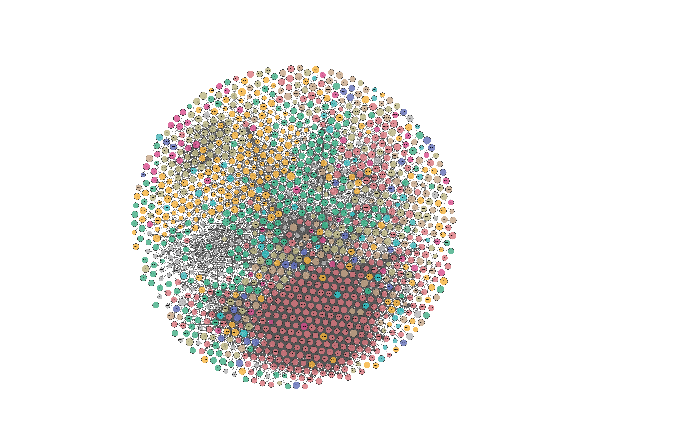
\includegraphics[width=5cm]{gfx/lod}}
\only<4-8>{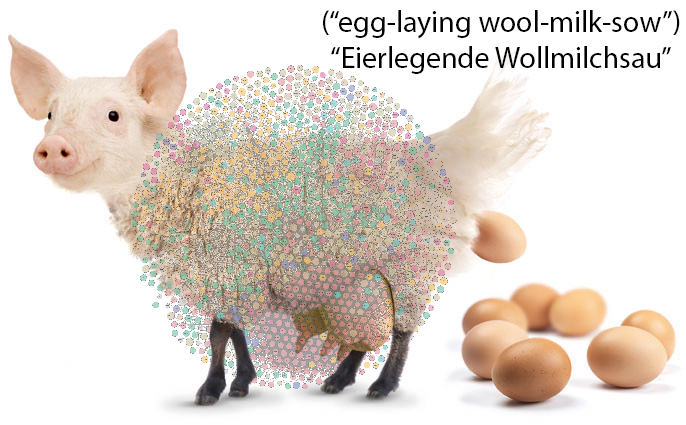
\includegraphics[width=5cm]{gfx/lod2}}
\only<9>{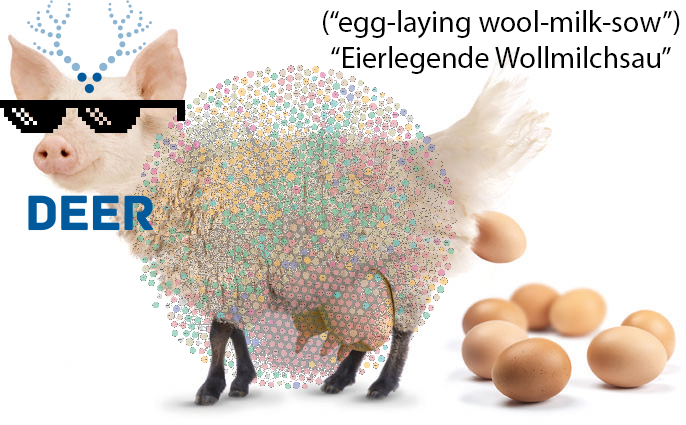
\includegraphics[width=5cm]{gfx/lod3}}
\end{textblock*}
\begin{itemize}
\item<1-> Linked Data is becoming more and more important
\item<2-> Linked Open Data (LOD) Cloud \footnote{Stats taken from \href{https://lodlaundromat.org}{LOD Laundromat}. Links estimated.}
{\begin{itemize}
  \item 650k datasets
  \item 38 billion triples
  \item $n\cdot10^6$ links ($10 < n < 1000$)
\end{itemize}}
\item<3->{Can we use this vast amount of data as is?}
\item<5-> Not so easy, due to
{\begin{itemize}
  \item<5-> limited resources
  \item<6-> unreliable SPARQL endpoints
  \item<7-> missing links
  \item<8-> application-specific ontologies
\end{itemize}}
\item<9-> RDF Dataset Enrichment to the rescue!
\end{itemize}
\end{frame}

%\subsection{RDF Dataset Enrichment}
\begin{frame}{\<DEER> - The RDF Dataset Enrichment Framework}
\begin{textblock*}{3cm}(13.1cm, -0.8cm) % {block width} (coords)

\includegraphics[width=3cm]{gfx/deer}
\end{textblock*}
\begin{itemize}
  \item<1-> \textbf{RDF Dataset Enrichment:} Adding\,/\,Deleting triples from an RDF Dataset
\end{itemize}
\uncover<2->{\begin{block}{Definition \textbf{Enrichment Operator}}
Let $\mathcal{D}$ be the set of all RDF Datasets.
We call a function $o : \mathcal{D}^n \to \mathcal{D}^m$ an \emph{Enrichment Operator}.
We call $n$ the in degree and $m$ the out degree of $o$.
\end{block}}
\end{frame}

\begin{frame}{\<DEER> - The RDF Dataset Enrichment Framework}
\only<1>{\begin{block}{Definition \textbf{Enrichment Graph}}
An Enrichment Graph $G=(V,E,L)$ is a Directed Acyclic Labeled Multigraph.\\
The root vertices $V_r={v \in V|\not\exists u \in V, (u, v) \in E}$ of an Enrichment Graph represent input RDF Datasets emitters.\\The leaf vertices $V_l={v \in V|\not\exists u \in V, (v, u) \in E}$ of an Enrichment Graph represent output RDF Datasets acceptors.\\The intermediate vertices $V_i=V\setminus V_r \setminus V_l $ represent Enrichment Operators.\\
The function $O : V \to \mathcal{O}$ maps vertices to the entities they represent.\\
An edge $(u, v) \in E \subseteq V \times V $ represents flow of data.\\The label function $L:E\to 2^{(\mathbb{N} \times \mathbb{N})}$ induces a mapping from the components of images and arguments of represented entities, i.e. for $e=(u,v)$, an entry of the label multiset $l\in L(e) = (i, j)$ establishes a flow of data from the $i$th component in the image of $O(u)$ to the $j$th argument of $O(v)$.
\end{block}}
\only<2>{\begin{block}{Definition \textbf{Enrichment Graph} (Continued)}
An Enrichment Graph $G=(V,E,L)$ with $\forall e\in E: |L(e)|=1$ is called an Enrichment Pipeline or a type 0 Enrichment Graph.\\
An Enrichment Graph $G=(V,E,L)$ with $\exists e\in E: |L(e)|>1 \land |V_r|=|V_l|=1$ is called a type 1 Enrichment Graph.\\
An Enrichment Graph $G=(V,E,L)$ with $\forall e\in E: |L(e)|>1 \land |V_r|>1 \land |V_l|=1$ is called a type 2 Enrichment Graph.\\
An Enrichment Graph $G=(V,E,L)$ with $\forall e\in E: |L(e)|>1 \land |V_r|>1 \land |V_l|>1$ is called a type 3 Enrichment Graph.
\end{block}}
\end{frame}

%\subsection{<DEER> }
\begin{frame}{Configuring \<DEER>}
\begin{itemize}
  \item Plugin architecture
  \item Most Enrichment Operators need parametrization
  \item Defining an Enrichment Graph requires expert knowledge
  \item $\to$ Use Machine Learning
\end{itemize}
\end{frame}

%\subsection{Objective of the Thesis}
\begin{frame}{Existing ML Algorithm in \<DEER>}
\begin{itemize}
  \item Learns type 1 Enrichment Graphs based on Refinement Operators
  \item Training data: RDF Datasets Source ($S$) and Target ($T$)
  \item Fitness Function: $F_1$ score over triples
  \item Iteratively construct Enrichment Graph $G$ from Set of all Enrichment Operators $\mathcal{O}$
  \item Set $G:=\textit{nil}, B:=S$
  \item Until Termination Criterion met:
  \begin{itemize}
    \item $\forall o\in\mathcal{O}: o\textit{.selfConfig}(B, T)$
    \item $G := G \circ \arg\max_{F_1(T, B')}\{o'\in\mathcal{O}|B'=(G \circ o')(B)\}$
    \item $B := G(B)$
  \end{itemize}
\end{itemize}
\end{frame}
\begin{frame}{Analysis of Existing ML Algorithm in \<DEER>}
\begin{itemize}
  \item Good theoretical properties \small{(finite, proper, complete, not redundant)}
  \item But several incorrect implicit assumptions
  \begin{itemize}
    \item $F_1$ score over triples is indicative for fitness $\lightning$
    \begin{itemize}
      \item Counterexample: Filtering first
    \end{itemize}
    \item Enrichment Operators are independent $\lightning$
    \begin{itemize}
      \item Counterexample: Linking $\to$ Dereferencing 
    \end{itemize}
    \item Training data always contains sufficient information for self-configuration $\lightning$
    \begin{itemize}
      \item possible, but not realistic
      \item at least as hard to satisfy as manual configuration
    \end{itemize}
  \end{itemize}
  \item $\to$ Objective of this thesis: develop new approach
\end{itemize}
\end{frame}
\begin{frame}{Derived Goals}
  The new Approach should:
\begin{enumerate}
  \item derive proper fitness function
  \item take interdependency of Enrichment Operators into account
  \item cope with incomplete information w.r.t. self-configuration
  \item be applicable for type 0, 1 \& 2 Enrichment Graphs
\end{enumerate}
\end{frame}
\section{Approach}
%\subsection{Guided Evolutionary Learning}
\begin{frame}{(1) Fixing the Fitness Function}
    \begin{itemize}
      \item Weight recall higher than precision ($F_2$ score)
      \item Linear combination of $F_2$ score over triples, URI resources \& literals
      \item Apply fuzzy matching to URI resources \& literals
    \end{itemize}
\end{frame}

\begin{frame}{(2) Leveraging Enrichment Operator Interdependency}
    \begin{itemize}
      \item avoid local minima $\to$ employ genetic programming  
      \item infer possible dependencies using top-down self-configuration
      \item recursive broadcast algorithm: $\textit{broadcast}(\mathcal{G},D_{\bot},D_{\top})$
      \begin{itemize}
      \item each $o$ assesses if $D_{\top}$ is a possible postcondition
      \item each $o$ reports a number between $0$ and $1$ based on its assessment
      \item if some termination criteria holds, return $\mathcal{G}$
      \item the Enrichment Operators reporting the highest $k$ values are chosen
      \item for each chosen Enrichment Operator $o_c$ call $\textit{broadcast}(\mathcal{G'}=\{G \circ o_c |G\in\mathcal{G}\},D_{\bot},o_c^{-1}(D_{\top}))$
      \end{itemize}
      \item started as: $\forall o\in\mathcal{O}: \textit{broadcast}(\{\},S,T)$
    \end{itemize}
\end{frame}

\begin{frame}{(3) Reconstructing Hidden Information for Self-Configuration}
    \begin{itemize}
      \item top-down self-configuration reconstructs hidden information!
    \end{itemize}
\end{frame}

\begin{frame}{(4) From Type 0 to Type 2}
\begin{itemize}
  \item Type 0: Base implementation
  \item Type 1: Extends Type 0
    \begin{itemize}
      \item Allow branching and merging in inital population generation
      \item Force merging at leafs
      \item Detect independent Enrichment Operators \& parallelize
    \end{itemize}
  \item Type 2: Theory not finished yet
\end{itemize}
\end{frame}

\section{Evaluation Setup}
\begin{frame}{Evaluation Setup}
\begin{itemize}
  \item find use cases for each Enrichment Graph type
  \item write manual configurations to generate training data
  \item run each experiment ten times
  \item record precision, recall, run time, logs
  \item $\to$ compare with baseline
  \item compare complexity of manual and learned Enrichment Graphs
\end{itemize}
\end{frame}

\section{Roadmap}
\begin{frame}{Roadmap}
\begin{itemize}
  \item Evaluation of Type 0: 22.02.
  \item Evaluation of Type 1: 01.03.
  \item Evaluation of Type 2: 15.03.
  \item Hand in thesis: 29.03.
  \item Final presentation: 12.04.
  \item Official due date: 07.05.
\end{itemize}
\end{frame}

\begin{frame}{Thank You for Your Attention}

\end{frame}



\end{document}
